%%%%%%%%%%%%%%%%%%%%%%%%%%%%%%%%%%%%%%%%%%%%%%%%%%%%%%%%%%%%%%%%%%%%%%%%%%%%%%%%
%Tutorial slides on Python.
%
% Author: FOSSEE 
% Copyright (c) 2009-2011, FOSSEE, IIT Bombay
%%%%%%%%%%%%%%%%%%%%%%%%%%%%%%%%%%%%%%%%%%%%%%%%%%%%%%%%%%%%%%%%%%%%%%%%%%%%%%%%

\documentclass[14pt,compress]{beamer}

% Modified from: generic-ornate-15min-45min.de.tex
\mode<presentation>
{
  \usetheme{Warsaw}
  \useoutertheme{infolines}
  \setbeamercovered{transparent}
}

\usepackage[english]{babel}
\usepackage[latin1]{inputenc}
%\usepackage{times}
\usepackage[T1]{fontenc}
\usepackage{pgf}

% Taken from Fernando's slides.
\usepackage{ae,aecompl}
\usepackage{mathpazo,courier,euler}
\usepackage[scaled=.95]{helvet}

\definecolor{darkgreen}{rgb}{0,0.5,0}

\usepackage{listings}
\lstset{language=Python,
    basicstyle=\ttfamily\bfseries,
    commentstyle=\color{red}\itshape,
  stringstyle=\color{darkgreen},
  showstringspaces=false,
  keywordstyle=\color{blue}\bfseries}

%%%%%%%%%%%%%%%%%%%%%%%%%%%%%%%%%%%%%%%%%%%%%%%%%%%%%%%%%%%%%%%%%%%%%%
% Macros
\setbeamercolor{emphbar}{bg=blue!20, fg=black}
\newcommand{\emphbar}[1]
{\begin{beamercolorbox}[rounded=true]{emphbar} 
      {#1}
 \end{beamercolorbox}
}
\newcounter{time}
\setcounter{time}{0}
\newcommand{\inctime}[1]{\addtocounter{time}{#1}{\tiny \thetime\ m}}

\newcommand{\typ}[1]{\lstinline{#1}}

\newcommand{\kwrd}[1]{ \texttt{\textbf{\color{blue}{#1}}}  }

%%% This is from Fernando's setup.
% \usepackage{color}
% \definecolor{orange}{cmyk}{0,0.4,0.8,0.2}
% % Use and configure listings package for nicely formatted code
% \usepackage{listings}
% \lstset{
%    language=Python,
%    basicstyle=\small\ttfamily,
%    commentstyle=\ttfamily\color{blue},
%    stringstyle=\ttfamily\color{orange},
%    showstringspaces=false,
%    breaklines=true,
%    postbreak = \space\dots
% }

%%%%%%%%%%%%%%%%%%%%%%%%%%%%%%%%%%%%%%%%%%%%%%%%%%%%%%%%%%%%%%%%%%%%%%
% Title page
\title[Advanced Sci Comp.]{Advanced Scientific Computing with
Python}
\subtitle{Virtualenv, Cython }

\author[FOSSEE] {FOSSEE}

\institute[IIT Bombay] {Department of Aerospace Engineering\\IIT Bombay}
\date[] {PyCon Asia-Pacific,\\
Singapore\\
June 9, 2011
}
%%%%%%%%%%%%%%%%%%%%%%%%%%%%%%%%%%%%%%%%%%%%%%%%%%%%%%%%%%%%%%%%%%%%%%

%\pgfdeclareimage[height=0.75cm]{iitmlogo}{iitmlogo}
%\logo{\pgfuseimage{iitmlogo}}


%% Delete this, if you do not want the table of contents to pop up at
%% the beginning of each subsection:
\AtBeginSubsection[]
{
  \begin{frame}<beamer>
    \frametitle{Outline}
    \tableofcontents[currentsection,currentsubsection]
  \end{frame}
}

\AtBeginSection[]
{
  \begin{frame}<beamer>
    \frametitle{Outline}
    \tableofcontents[currentsection,currentsubsection]
  \end{frame}
}

% If you wish to uncover everything in a step-wise fashion, uncomment
% the following command: 
%\beamerdefaultoverlayspecification{<+->}

%%\includeonlyframes{current,current1,current2,current3,current4,current5,current6}

%%%%%%%%%%%%%%%%%%%%%%%%%%%%%%%%%%%%%%%%%%%%%%%%%%%%%%%%%%%%%%%%%%%%%%
% DOCUMENT STARTS
\begin{document}

\begin{frame}
  \maketitle
\end{frame}

%% \begin{frame}
%%   \frametitle{Outline}
%%   \tableofcontents
%%   % You might wish to add the option [pausesections]
%% \end{frame}

\section{Virtualenv}


\begin{frame}
  \frametitle{Motivation}
  \begin{itemize}

      \item Need to install Python packages

      \item No root access

      \item Don't want to mess up system

      \item Create ``isolated'' environment

      \item PyPI
  
  \end{itemize}

\end{frame}

\begin{frame}[fragile]
  \frametitle{Virtualenv}

  \begin{itemize}
    \item  \url{www.virtualenv.org} 

    \item \url{pypi.python.org/pypi/virtualenv}

    \item Either install virtualenv 
        
    \item Oe use the \typ{virtualenv.py}

  \end{itemize}

  \begin{lstlisting}
$ easy_install virtualenv
  \end{lstlisting}
Or download tarball and
  \begin{lstlisting}
$ python setup.py install \
>  [--prefix=/usr/local]
  \end{lstlisting}

\end{frame}

\begin{frame}[fragile]
  \frametitle{Environments}
Creation:

  \begin{lstlisting}
$ python virtualenv.py ENV
  \end{lstlisting}

  \begin{itemize}
      \item \typ{ENV} is a directory name of your choice
      \item Self-contained universe
      \item By default (optional) inherits system packages
      \item Look in \typ{ENV/bin} (or \typ{ENV\\Scripts})

      \item Look in \typ{ENV/lib} (or \typ{ENV\\Lib})
  \end{itemize}

\end{frame}

\begin{frame}[fragile]
  \frametitle{Activation}

  \begin{lstlisting}
# Activation (Linux/Mac OSX)
$ source ENV/bin/activate

$ ENV\Scripts\activate.bat

# Deactivate
(ENV)$ deactivate

$ ENV\Scripts\deactivate.bat
  \end{lstlisting}
  \vspace*{0.1in}
  I prefer to activate in \typ{.bash_profile}
\end{frame}

\begin{frame}[fragile]
  \frametitle{Usage}
  \begin{lstlisting}
(ENV)$ python # this is ENV/bin/python

(ENV)$ easy_install my_fav_package
(ENV)$ pip install my_fav_package
# All above install into ENV.

(ENV)$ python setup.py install
# Also installs into ENV

  \end{lstlisting}

\end{frame}

\begin{frame}[fragile]
  \frametitle{Usage}
  \vspace*{-1em}
  \begin{lstlisting}
(ENV)$ deactivate
$ python virtualenv.py ANOTHER
(ANOTHER)$ source ANOTHER/bin/activate
(ANOTHER)$ pip install PKG
# installs in ANOTHER

(ANOTHER)$ deactivate
$ source ENV/bin/activate

# To remove ANOTHER
$ rm -rf ANOTHER
\end{lstlisting}

That is it! Easy, and very convenient

\inctime{15}

\end{frame}

\section{Cython}

\begin{frame}
  \frametitle{Motivation}
  \begin{itemize}

      \item Pure Python can be very slow

      \item Not trivial to write C-extensions

      \item Interfacing to C libraries not too easy 

  \end{itemize}

\end{frame}

\begin{frame}
  \frametitle{Introduction}
  \begin{itemize}
    
    \item Python-based language

    \item Optional static typing

    \item Call external C libraries

    \item Python to C compiler

    \item \alert{``Cython is Python with C-data-types''}

    \item \url{cython.org}

    \item \url{docs.cython.org}
    
    \item 500x speedup is possible!

  \end{itemize}

\end{frame}

\begin{frame}
    \frametitle{Basic structure}

    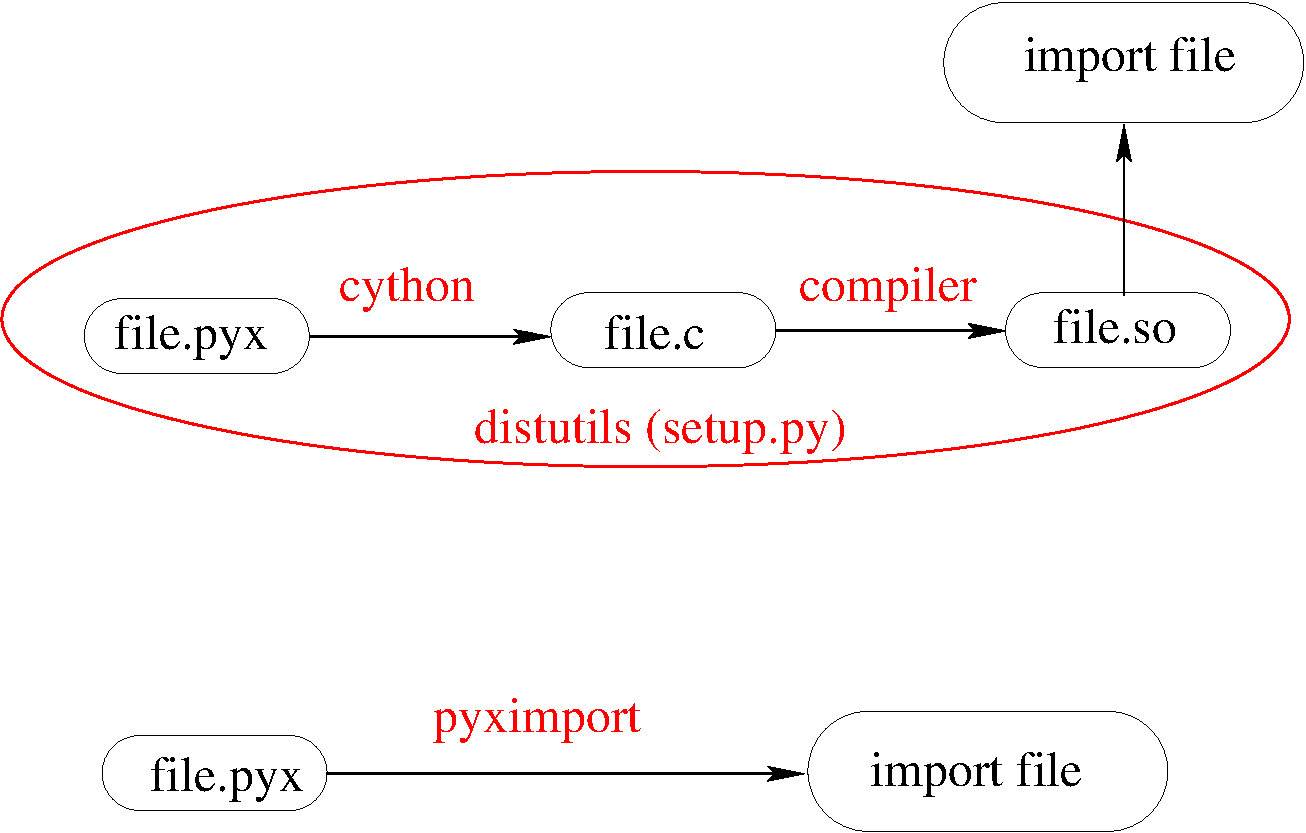
\includegraphics[height=3in]{data/cython}

\end{frame}

\begin{frame}[fragile]
    \frametitle{Simple example}
\begin{lstlisting}
# -- hello.pyx --
def hello(name):
    print("Hello %s!"%name)
# EOF

$ ipython
In []: import pyximport
In []: pyximport.install()
In []: import hello
In []: hello.hello('PyCon')
Hello PyCon!
\end{lstlisting}

\end{frame}

\begin{frame}[fragile]
    \frametitle{Simple \typ{setup.py}}
\begin{lstlisting}
# -- setup.py --
from setuptools import setup
from Cython.Distutils import build_ext
from numpy.distutils.extension import \ 
    Extension
setup(
    cmdclass = {'build_ext': build_ext},
    ext_modules = [Extension("hello", 
                   ["hello.pyx"])
                  ]
)
# EOF
\end{lstlisting}

\end{frame}

\begin{frame}[fragile]
    \frametitle{Compiling the code}
\begin{lstlisting}
$ python setup.py build_ext --inplace
# ...
$ ipython
In []: import hello
In []: hello.hello('PyCon')
Hello PyCon!
\end{lstlisting}

\end{frame}

\begin{frame}[fragile]
    \frametitle{Meaningful example: Phase 0}
\begin{lstlisting}
# -- quad0.pyx --
from math import sin
def f(x):
    return sin(x**2)

def integrate(a, b, N):
    s = 0
    dx = float(b-a)/N
    for i in range(N):
        s += f(a+i*dx)
    return s * dx
\end{lstlisting}

\end{frame}

\begin{frame}[fragile]
    \frametitle{Phase 1}
    \vspace*{-0.2in}
\begin{lstlisting}
# -- quad1.pyx --
from math import sin
\end{lstlisting}
\lstset{backgroundcolor=\color{yellow}}
\begin{lstlisting}
def f(double x):
\end{lstlisting}
\lstset{backgroundcolor=\color{white}}
\vspace*{-1ex}
\begin{lstlisting}
    return sin(x**2)
\end{lstlisting}
\lstset{backgroundcolor=\color{yellow}}
\begin{lstlisting}
def integrate(double a, double b, int N):
    cdef int i
    cdef double s, dx
\end{lstlisting}
\lstset{backgroundcolor=\color{white}}
\vspace*{-1ex}
\begin{lstlisting}
    s = 0.0
    dx = float(b-a)/N
    for i in range(N):
        s += f(a+i*dx)
    return s * dx
\end{lstlisting}

\end{frame}

\begin{frame}[fragile]
    \frametitle{Timing}
\begin{lstlisting}
In []: import quad0
In []: %timeit quad0.integrate(0,1,10000)
100 loops, best of 3: 3.45 ms per loop

In []: import quad1
In []: %timeit quad1.integrate(0,1,10000)
100 loops, best of 3: 2.24 ms per loop
\end{lstlisting}
Not much.
\end{frame}

\begin{frame}[fragile]
    \frametitle{Cython annotation}
\begin{lstlisting}
$ cython -a quad1.pyx

$ firefox quad1.html
\end{lstlisting}
Very handy!

\inctime{15}
\end{frame}


\begin{frame}[fragile]
    \frametitle{Phase 2}
\begin{lstlisting}
# -- quad2.pyx --
from math import sin
cdef double f(double x) except *:
    return sin(x**2)
# ...
\end{lstlisting}
Could also use \typ{cpdef} instead

\begin{lstlisting}
In []: %timeit quad2.integrate(0,1,10000)
1000 loops, best of 3: 1.25 ms per loop
\end{lstlisting}
Looks like calling a Python function is slow.

\end{frame}

\begin{frame}[fragile]
    \frametitle{Phase 3: external C functions}
    Calling \typ{math.h}
\begin{lstlisting}
# -- quad3.pyx --
cdef extern from "math.h":
    double sin(double)

cdef double f(double x):
    return sin(x**2)
# ...
\end{lstlisting}

\begin{lstlisting}
In []: %timeit quad3.integrate(0,1,10000)
1000 loops, best of 3: 276 us per loop
\end{lstlisting}
\end{frame}


\begin{frame}[fragile]
    \frametitle{Extension classes}
    \small
\begin{lstlisting}
cdef class Function:
    cpdef double eval(self, double x) except *:
        return 0

cdef class SinOfSquareFunction(Function):
    cpdef double eval(self, double x) except *:
        return sin(x*x)

\end{lstlisting}
\pause
\begin{lstlisting}
def integrate(Function f, double a, double b, 
              int N):
    # ...
    for i in range(N):
\end{lstlisting}
\lstset{backgroundcolor=\color{yellow}}
\vspace*{-1em}
\begin{lstlisting}
        s += f.eval(a+i*dx)
\end{lstlisting}
\lstset{backgroundcolor=\color{white}}
\vspace*{-1em}
\begin{lstlisting}
    return s * dx
\end{lstlisting}
\end{frame}

\begin{frame}
    \frametitle{Extension classes}
    \begin{itemize}
        \item Can be extended in Python
        \item No multiple inheritance
        \item Cannot subclass Python class in Cython
        \item Can have typed attributes
        \item More info: \url{docs.cython.org}
    \end{itemize}
    \inctime{10}
\end{frame}

\begin{frame}[fragile]
    \frametitle{NumPy support}
\begin{lstlisting}
import numpy as np
cimport numpy as np

# Declare numpy arrays.
cdef np.ndarray arr

# Better still
cdef np.ndarray[np.int64_t, ndim=2] arr

\end{lstlisting}

\end{frame}

\begin{frame}[fragile,allowframebreaks]
    \frametitle{Full example}
    \small
\begin{lstlisting}
import numpy as np
\end{lstlisting}
\lstset{backgroundcolor=\color{yellow}}
\begin{lstlisting}
cimport cython
cimport numpy as np
@cython.boundscheck(False)
def mandel_cy(int h, int w, int maxit=20):
\end{lstlisting}
\lstset{backgroundcolor=\color{white}}
\vspace*{-1em}
\begin{lstlisting}
    """Mandelbrot set ..."""
\end{lstlisting}
\vspace*{-1em}
\lstset{backgroundcolor=\color{yellow}}
\begin{lstlisting}
    cdef np.ndarray[np.complex128_t, ndim=2] c
    cdef np.ndarray[np.int64_t, ndim=2] output
    cdef int i, j, k
    cdef double complex c0, z
\end{lstlisting}
\lstset{backgroundcolor=\color{white}}
\begin{lstlisting}
    x, y = np.ogrid[-2:0.8:w*1j, -1.4:1.4:h*1j]
    c = x+y*1j
    output = np.zeros((w, h), dtype=int) + maxit
    for i in range(h):
        for j in range(w):
            z = c[i,j]
            c0 = c[i,j]
            for k in xrange(maxit):
                z = z**2 + c0
\end{lstlisting}
\vspace*{-1em}
\lstset{backgroundcolor=\color{yellow}}
\begin{lstlisting}
                if (z*z.conjugate()).real > 4.0:
\end{lstlisting}
\vspace*{-1em}
\lstset{backgroundcolor=\color{white}}
\begin{lstlisting}
                    output[i, j] = k
                    break
    return output.T
\end{lstlisting}
\end{frame}

\begin{frame}[fragile,plain]
    \frametitle{The result}
\begin{lstlisting}
In []: from mandel_cy import mandel_cy
In []: o = mandel_cy(1024,1024)
In []: imshow(o)
\end{lstlisting}
\vspace*{-1em}
\begin{center}
    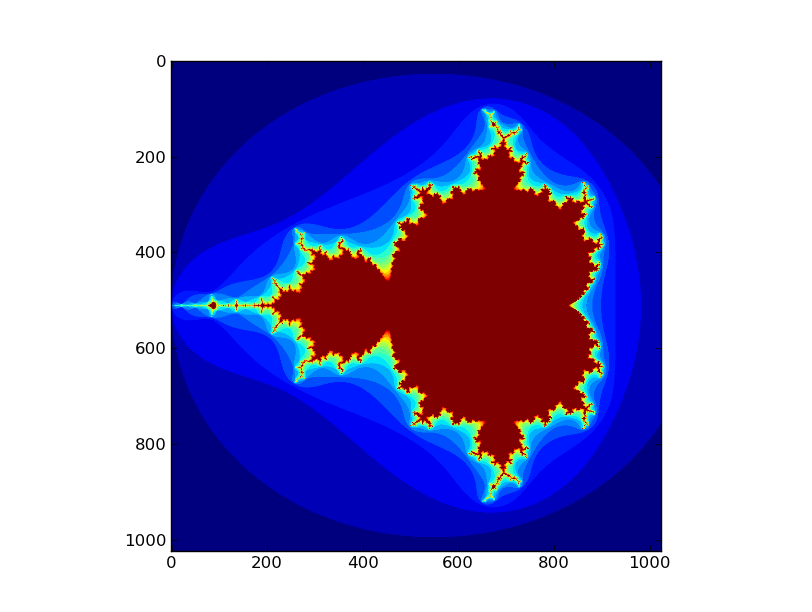
\includegraphics[height=2.5in]{data/mandelbrot}
\end{center}
\end{frame}

\begin{frame}[fragile]
    \frametitle{Timing}
    \begin{lstlisting}
In []: %timeit mandel_py(256, 256)
1 loops, best of 3: 2.96 s per loop

In []: %timeit mandel_np(256,256)
10 loops, best of 3: 42.5 ms per loop

In []: %timeit mandel_cy(256,256)
100 loops, best of 3: 3.95 ms per loop
    \end{lstlisting}
A whopping 700x speedup!
\end{frame}

\begin{frame}
    \frametitle{Additional points}
    \begin{itemize}
        \item \typ{.pxd} files
        \item Compiler directives:
            \begin{itemize}
                \item \typ{nonecheck}
                \item \typ{boundscheck}
            \end{itemize}
    \end{itemize}
    \inctime{10}
\end{frame}


\end{document}

